\documentclass[margin=0.1cm]{standalone}

%\usepackage{stix2}
\usepackage[]{tgheros}
\renewcommand{\familydefault}{\sfdefault}
\usepackage{arevmath}
\usepackage[italic]{mathastext}
\usepackage[T1]{fontenc}


\usepackage{pgfplots}
\pgfplotsset{compat=1.17}
\usepgfplotslibrary{units}
\usepackage{siunitx}

\begin{document}
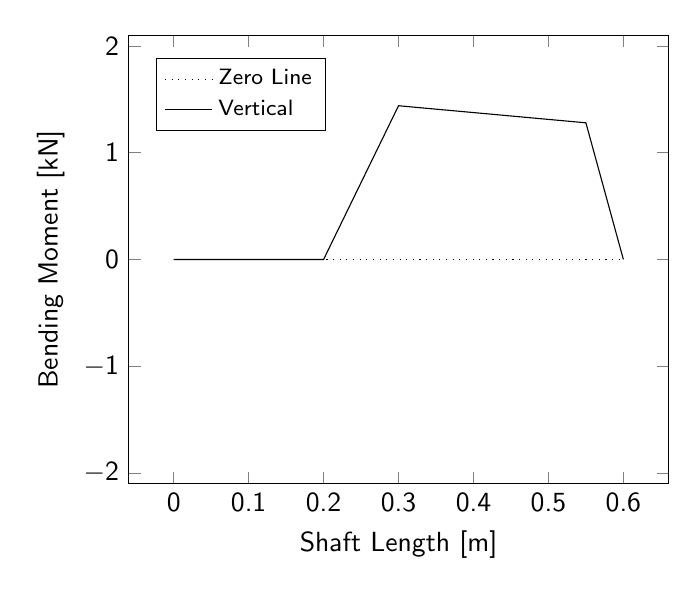
\begin{tikzpicture}
    \begin{axis}[
        xlabel = Shaft Length,
        ylabel = Bending Moment,
        use units,
        x unit=\si{\metre},
        y unit=\si{\kilo\newton},
        legend style={at={(0.05,0.95)},anchor=north west, font=\footnotesize},
        legend cell align=left,
        ymin={-2.1},
        ymax={2.1}
    ]
    
    \addplot[color=black, dotted] coordinates {
        (0,0)
        (0.6,0)
    };
    
    \addplot[color=black] coordinates {
        (0,0)
        (0.2,0)
        (0.3, 1.44)
        (0.55, 1.28)
        (0.6, 0)
    };
    
    \legend{Zero Line, Vertical}
    
    \end{axis}
\end{tikzpicture}
\end{document}